\documentclass{article}
\usepackage{amsmath}
\usepackage{amsthm}
\usepackage{amsfonts}
\usepackage{amssymb}
\usepackage{bbold}
\usepackage{dsfont}
\usepackage{graphicx}
\usepackage{cleveref}
\usepackage{bm}
\usepackage{booktabs}
\usepackage{siunitx}
\usepackage{xcolor}
\usepackage{pdfpages}
\usepackage[utf8]{inputenc}
\usepackage[english]{babel}
\newtheorem{definition}{Definition}
\newtheorem{example}{Example}
\newcommand{\exP}[1]{\mathrm{e}^{#1}}
\newcommand{\dif}{\mathrm{d}}
\renewcommand{\vec}[1]{\mathbf{#1}}
\newcommand{\pdagger}{{\phantom{\dagger}}}
\newcommand{\state}[1]{\vert #1\rangle}
\newcommand{\cstate}[1]{\langle #1\vert}
\newcommand{\outerp}[2]{\vert #1\rangle\!\langle #2 \vert}
\newcommand{\tr}[1]{\mathrm{tr}\left\{#1\right\}}
\newcommand{\trs}[2]{\, \mathrm{tr}_{#1}\{#2\}}
\newcommand{\expc}[3]{\langle #1\vert #2 \vert #3\rangle}
\usepackage[doi=false,url=false,isbn=false,backend=bibtex,style=nature,natbib=true,sorting=none]{biblatex}
\bibliography{bib.bib}
\usepackage{geometry}
\geometry{
	a4paper,
	total={170mm,257mm},
	left=15mm,
	right=15mm,
	top=15mm,
}
\usepackage{kbordermatrix}
\begin{document}
\title{Addition to previous meetings}
\author{Rudolf}
\maketitle
\section{Rank ''dynamics'' in Subotniks model (vanishing molecule-lead coupling)}
\begin{figure}[!h]
	\centering
	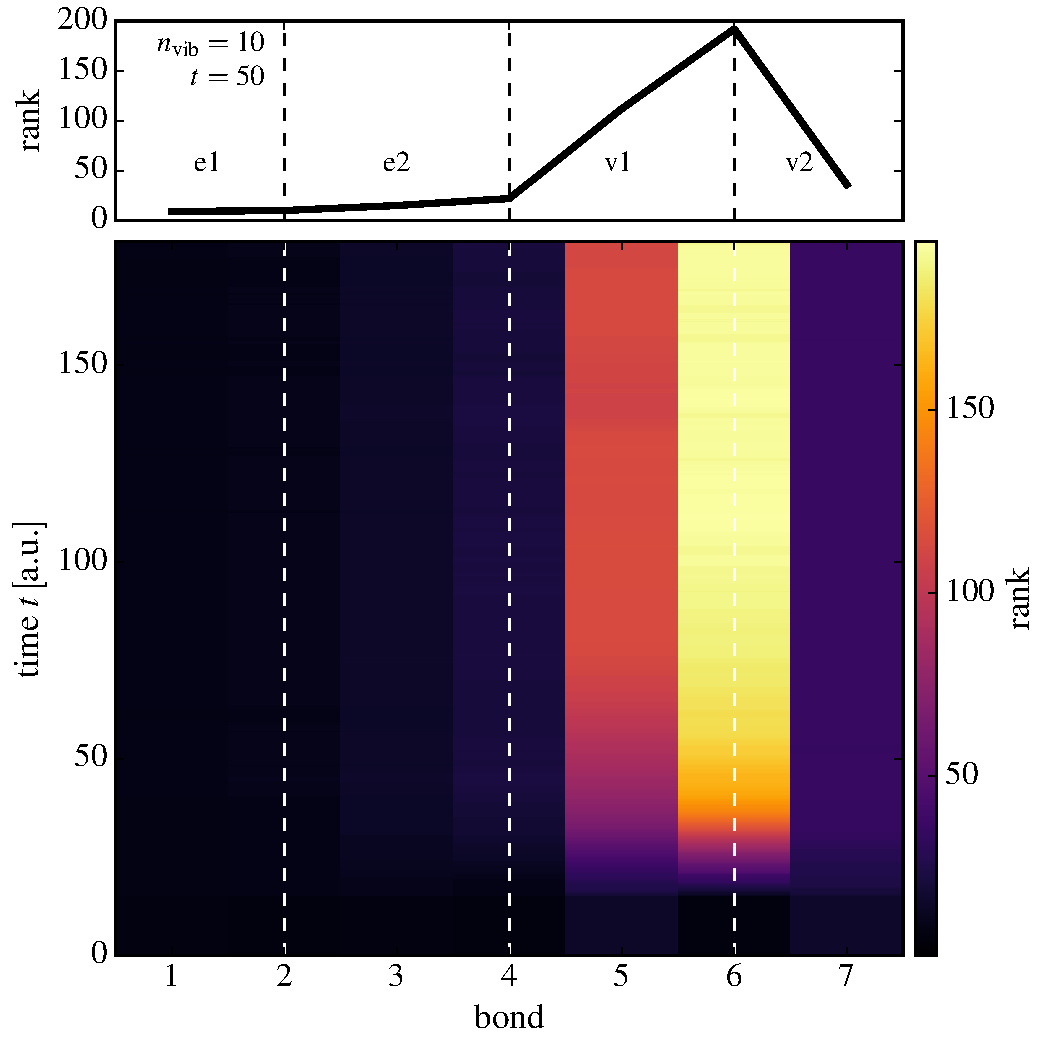
\includegraphics[width=0.8\textwidth]{figs/Iso_Subotnik_noSpin_nv10_rank.pdf}
\end{figure}
\clearpage
\section{Addition to Ehrenfest paper}
\subsection{Phase space trajectory (randomly sampled initial condition)}
\begin{figure}[!h]
	\centering
	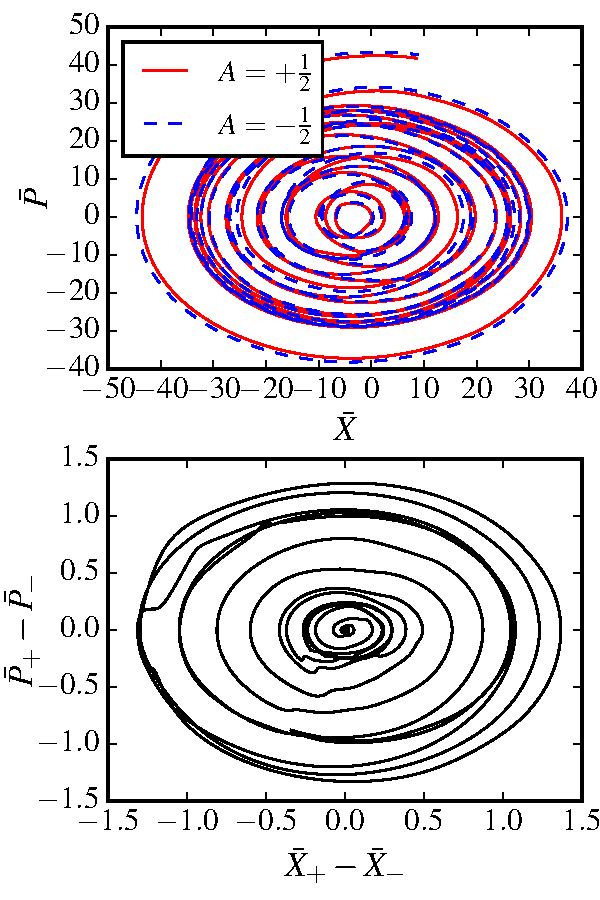
\includegraphics[width=0.8\textwidth]{figs/PhaseSpace_L5_init_random.pdf}
\end{figure}
\subsection{Plot combining time-dependent spectrum, electronic population, vibrational and molecule-lead coupling}
\begin{figure}[!h]
	\centering
	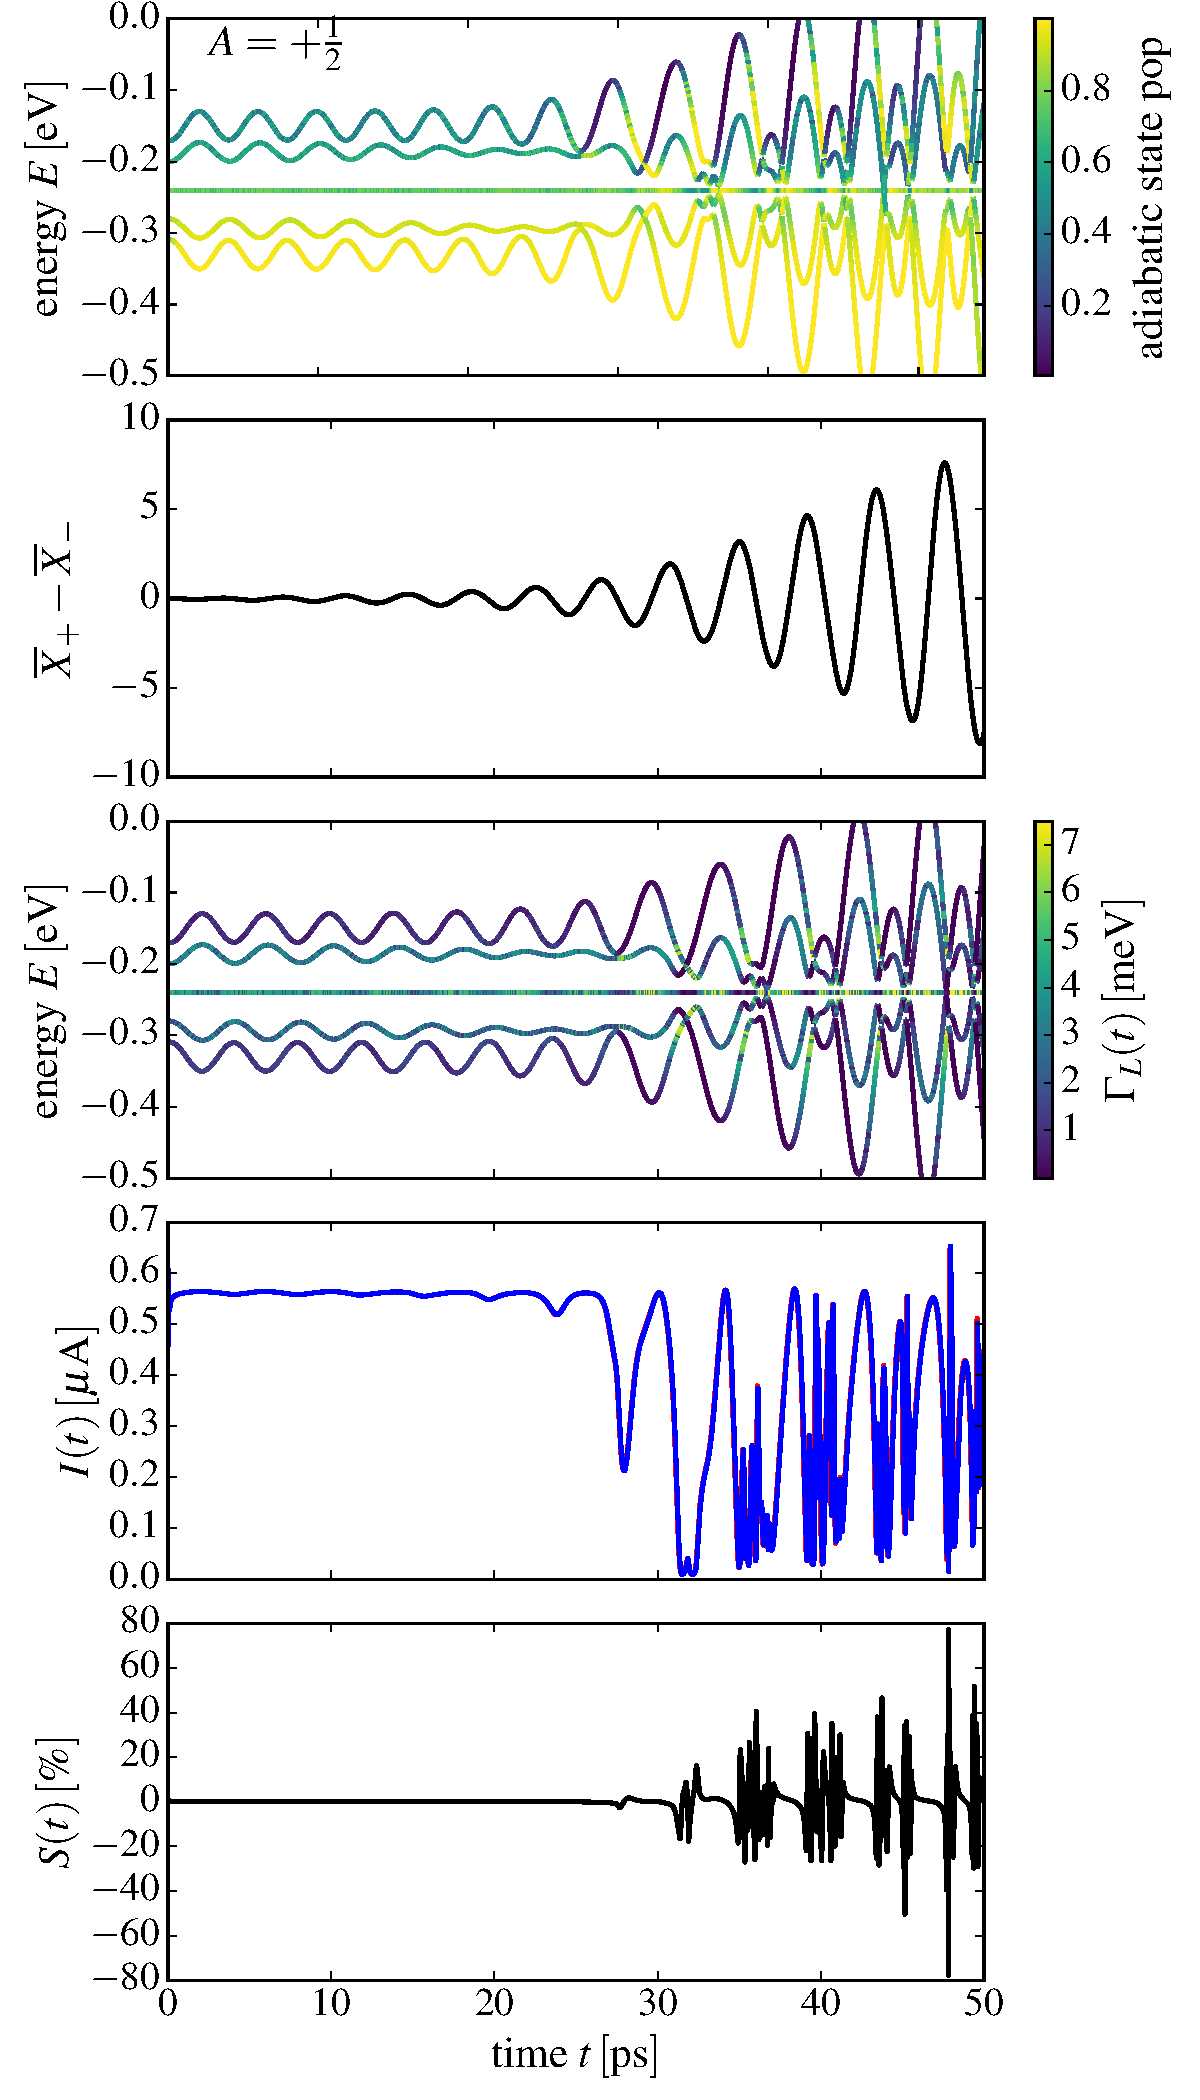
\includegraphics[width=0.82\textwidth]{figs/L1x5_elec_es_spec_Xdif_gamma_td_cur_P_singleTraj.pdf}
\end{figure}
\clearpage
\subsection{Combined picture}
\begin{figure}[!h]
	\centering
	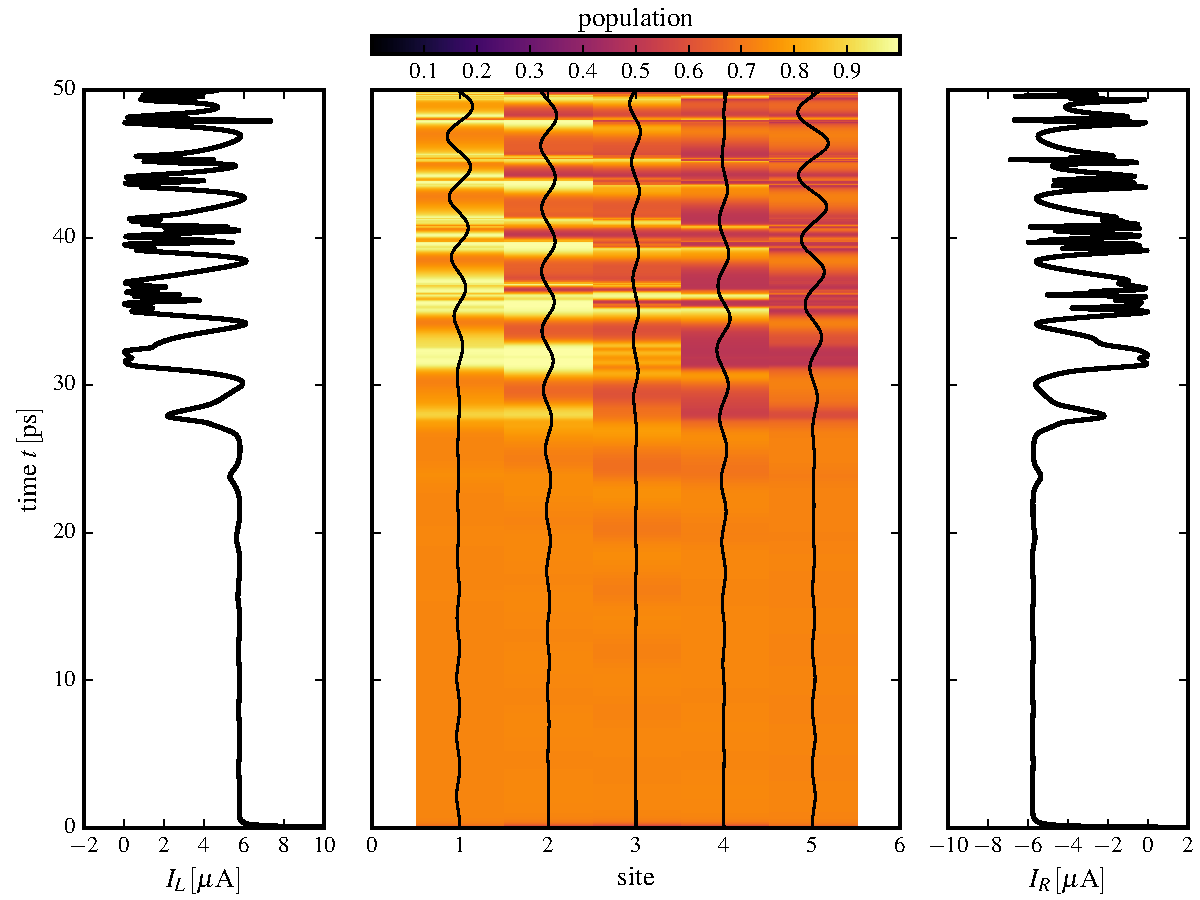
\includegraphics[width=0.8\textwidth]{figs/Cur_nd_phonons_L1x5.pdf}
\end{figure}

\end{document}


